% !TeX root = ./thesis.tex
% !TeX encoding = UTF-8
% !TeX spellcheck = en_GB

\documentclass[print]{mystyle}

% Set up metadata
\author{Wouter Duverger}
\title{Polarisation-resolved super-resolution microscopy}
\date{May 10, 2021}

% Register figure folders (twice, for Windows and Linux)
\graphicspath{
	{../figures_generated}
	{../figures_generated/}
	{../figures_other}
	{../figures_other/}
}

% Shorthands
\newcommand{\qwp}{{\lambda/4}}
\newcommand{\hwp}{{\lambda/2}}
\newcommand{\Eox}{E_{0x}}
\newcommand{\Eoy}{E_{0y}}
\newcommand{\na}{\mathrm{NA}}
\newcommand{\exc}{\mathit{ex}}
\newcommand{\dep}{\mathit{dep}}
\newcommand{\emm}{\mathit{em}}
\newcommand{\unitvec}[1]{\hat{\vb{#1}}}
\newcommand{\se}{\mathit{se}}

%\includeonly{text/results}

\begin{document}

% !TeX spellcheck = en_GB
{
\pagestyle{empty}

\begin{tikzpicture}[remember picture,overlay]
	\node[inner sep=0pt] at (current page.center) {\includegraphics[page=1]{coverpage_g5.pdf}};
\end{tikzpicture}

\clearpage

\begin{titlepage}
	
	\frutigerfont
	
	\begin{center}

		
		{\Huge \garamondfont \thetitle}
		
		\smallskip
		by
		\bigskip
		
		{\Large \garamondfont \theauthor}
		
		\bigskip
		\bigskip
		
		This thesis is conducted in partial fulfilment of the requirements for the degree of 
		
		\bigskip
		
		{MSc in Physics} \\
		Biological Physics and Computational Biology,
		
		\bigskip
		
		at the NanoLund Centre for Nanoscience, Lund University,\\
		to be defended publicly on \todo{May ??, 2021}.
		
		
		\vspace{5cm}
		
		\vfill
		\begin{tabular}{ll}
			Project duration & 4 months (full-time equivalent)\\
			Supervision & Prof. Dr. Jonas Tegenfeldt\\
			Daily supervision & Dr. Jason Beech\\
			Examiner & Prof. Dr. Edouard Berrocal
		\end{tabular}
	
		\bigskip
	
		Cover image: artefacts of an old actin-phalloidin stained sample.
	
		\vspace{2cm}
		
		\includegraphics[width=0.5\linewidth]{nanolund_logotype.pdf}
	
	
	\end{center}
\end{titlepage}

%\cleardoublepage
%
%{
%\raggedleft
%
%\vspace*{\fill}
%
%
%``Space separates bodies, not minds.''\\
%-- Erasmus of Rotterdam
%
%\vspace*{\fill}
%
%
%}
%
%\cleardoublepage

}
	
\frontmatter

	\chapter*{Abstract}

\todo{to do}
	
	\renewcommand{\contentsname}{Table of Contents}
	\tableofcontents
	\addcontentsline{toc}{chapter}{Table of Contents}	
	
	% !TeX spellcheck = en_GB
\chapter{Nomenclature}

\begin{tabular}{ll}
	APD       & Avalanche photodetector                                             \\
	AOM       & Acousto-optical modulator                                           \\
	au        & Arbitrary units                                                     \\
	CCD       & Charge-coupled device                                               \\
	DAPI     & 4',6-diamidino-2-phenylindole                                       \\
	DNA       & Deoxyribonucleic acid                                               \\ %	FC        & Filter cube
	% FC      & Filter cube                                                         \\
	FLIM      & Fluorescence lifetime imaging microscopy                            \\
	FOV       & Field of view                                                       \\
	FWHM      & Full width at half maximum                                          \\
	GFP       & Green fluorescent protein                                           \\
	HSV       & Hue, saturation, value                                              \\
	HWP       & Half-wave plate                                                     \\
	MPE       & Maximum permissible exposure                                        \\
	NA        & Numerical aperture                                                  \\
	OD        & Optical density                                                     \\
	          & (an OD2 filter reduces the light intensity by a factor of $ 10^2 $) \\
	PBS       & Polarising beam splitter                                            \\
	PMT       & Photomultiplier tube                                                \\
	PSF       & Point spread function                                               \\
	pSTED     & Polarisation-dependent stimulated emission depletion microscopy      \\
	QWP       & Quarter-wave plate                                                  \\
	ROI      & Region of interest                                                  \\
	SARS-Cov2 & Severe acute respiratory syndrome coronavirus 2                     \\
	SiR       & Silicon-rhodamine                                                   \\
	SLM       & Spatial light modulator                                             \\
	SNR       & Signal-to-noise ratio                                               \\
	STED      & Stimulated emission depletion  microscopy                           \\
	TCSPC     & Time-correlated single photon counter
\end{tabular}

\mainmatter

	% !TeX spellcheck = en_GB
\chapter{Introduction}

\begin{itemize}
	\item Molecular biology has had a great impact on our standards of living. There are a ton of diseases out there, and by studying how they work, we can (a) learn how cells and organisms function, and (b) propose certain treatments. Example: use amyloid aggregation to fight cancer.
	
	\item One interesting disease is caused by the Yersinia genus. Yersinia pestis is a species that caused the plague, which killed a third of the people living in europe and the plague of justinian. Vaccinations are available and incidence is low (600 cases per year worldwide), so low clinical importance currently.
	
	\item However, interesting mode of action. Actin filaments are broken down, revealing small self-organising micropatterns of actin left. Studying this might lead to new fundamental knowledge of cell function. (Ultimate goal of this research programme.)
	
	\item Current goal: set up a microscope system to study this disease, marrying super resolution microscopy and polarisation microscopy.
	
	Microscopy - imaging structures at microscopic scales - is a wide and varied field. It is widely accepted to have began in the sixteen-hundreds, with Antoni van Leeuwenhoek's discovery of bacteria and other single-celled organisms \cite{VanZuylen1981}. After that, microscopes have been getting higher resolution, but as lenses got better and better, they were not the resolution bottleneck any more. Specifically, in 1873, Ernst Abbe determined that the best possible focus that a microscope can reach is limited by the wavelength of the light used \cite{Abbe1873}. This meant that the microscopes of the time were limited to a resolution of roughly 400 nm (assuming focused visible white light). It was long believed that the Abbe limit was a fundamental limit of nature, and that the only way around it was by using light of a different wavelength. This is one of the reasons for the development of electron microscopes \cite{Smith2008}, as quantum mechanics explains that accelerated electrons have much shorter wavelength than visible light. 
	
	Fluorescence microscopy is an invaluable tool in modern biology \cite{Danial2016}. Unlike other methods, it is able to tag specific protein species and other relevant molecules in the cell with a fluorescent label. There are thousands of small organic fluorescent labels, and more are being developed \cite{Zhang2002, Resch-Genger2008}. The introduction of GFP and other fluorescent proteins was a remarkable development in the field, as labels can now be genetically fused to proteins of interest \cite{Shaner2005, Matlashov2020}. There were over thirty thousand papers collected in the PubMed database that mentioned fluorescence in the year 2020 alone.
	
	\item Super resolution (STED) was already set up and had polarisation capabilities, but were never used. My main contributions lie in figuring out what all components do, how to characterise them etc. Most of that will be found in the Background and Methods sections.
	
	\item Another big part of work was developing a new polarisation microscopy method (pSTED) to improve the angular resolution of a polarisation microscope. Relate pSTED to a figure in the Yersinia pattern paper.
	
\end{itemize}
	% !TeX spellcheck = en_GB
\chapter{Background}

\todo{Why do we want to see small things?}

Microscopy - imaging structures at microscopic scales - is an extremely wide and varied field. It is widely accepted to have began in the sixteen-hundreds, with Antoni van Leeuwenhoek's discovery of bacteria and other single-celled organisms \todo{ref}. After that, microscopes have been getting higher resolution, but as lenses got better and better, they were not the resolution bottleneck any more. Specifically, in 1873, Ernst Abbe determined that the best possible focus that a microscope can reach is limited by the wavelength of the light used \todo{ref}. This meant that the microscopes of the time were limited to a resolution of roughly 400 nm (assuming focused visible white light). It was long believed that the Abbe limit was a fundamental limit of nature, and that the only way around it was by using light of a different wavelength. This is one of the reasons for the development of electron microscopes \todo{ref}, as quantum mechanics postulates that accelerated electrons have much shorter wavelength than visible light. 

\section{Diffraction-limited microscopy}

\todo{Fluorescence microscopy is great, but was limited in resolution until recently.} I will discuss two ways to get around this problem. The first is indirect and requires playing with a new aspect of light (polarisation) that allows you to get information about structures that you cannot see. The second (STED microscopy) directly increases the image resolution. The excitation light is still limited to the Abbe limit, but we add another laser to effectively improve our focusing.

\section{Polarisation microscopy}

The wave nature of light might limit the resolution of a microscope, but it can also be exploited in our favour. Light polarisation can inform on the orientation of structures in a sample that are smaller than the diffraction limit. Among other things, this has been used to measure how the structure of DNA changes when it is subject to a strong stretching force, how integrin proteins respond to an applied force and measure the order of molecules embedded in the cell membrane, among others \cite{Backer2019, Nordenfelt2017, Swaminathan2017, Brasselet2013}. In this section, I will first introduce the concept of light polarisation, then discuss how it can be used in a microscope, and finally mention some optical components that affect the light polarisation, which are crucial to conducting a polarisation microscopy experiment.

\paragraph{The polarisation ellipse.} Remember that light is a transverse electromagnetic wave. This means that there are oscillations of the electric and magnetic fields along the path of a light ray, and that these oscillations are orthogonal to the propagation direction. In other words, if the light propagates along $\vec{k}$, the electric and magnetic fields $\vec{E}$ and $\vec{B}$ must satisfy $ \vec{E} \cdot \vec{k} = \vec{B} \cdot \vec{k} = 0$. (The fields themselves are also orthogonal to each other, so we can neglect $ \vec{B} $ without compromising our analysis.)

For the sake of simplicity, let's consider a ray propagating in the $ z $ direction. The electric field at any point in space and time can be written as
\begin{align}
	E_x(z, t) &= \Eox \cos(kz-\omega t + \phi_x),\\
	E_y(z, t) &= \Eoy \cos(kz-\omega t + \phi_y).
\end{align}
where $ \vec{E}_0 $ is the amplitude of the oscillation, $ k $ is the wavenumber (the length of $ \vec{k} $), $ \omega $ is the radial frequency and $ \phi $ is an arbitrary phase. Note that the wavenumber and the frequency are related to each other through the speed of light $ c $, since $ \omega = kc$. Note that the $ x $ and $ y $ components can have a phase difference.

Letting $ \delta = \phi_y-\phi_x $, it can be shown that 
\begin{equation}
	\left(\frac{E_x}{\Eox}\right)^2 - 2\cos\delta\frac{E_x}{\Eox}\frac{E_y}{\Eoy} + \left(\frac{E_y}{\Eoy}\right)^2 = \sin^2\delta.
\end{equation}
This is the equation for an ellipse. That means that, at any point in time, the point $ (E_x, E_y) $ lies on the ellipse defined by the equation above, which is called the polarisation ellipse. The ellipse is characterised by $ \Eox $, $ \Eoy $ and $ \delta $:
\begin{itemize}
	\item if $ \Eox = 0 $, the ray is said to be linearly polarised in the $ y $ direction, and vice versa,
	\item if neither are equal to 0, but they are in phase (meaning $ \delta=0 $), the light is still polarised, at an angle $ \psi = \arctan(\Eoy/\Eox) $ to the $ x $ axis,
	\item if the amplitudes in $ x $ and $ y $ are equal, and $ \delta = \pm \pi/4 $, then the light is circularly polarised. If $ delta $ is positive (negative), the polarisation is said to be right-handed (left-handed). \todo{replace this list by table}
\end{itemize}

\begin{table}
	\centering
	\begin{tabular}{lllll}
		\toprule
		Polarisation state      & $ \Eox $ & $ \Eoy $ & $ \delta $ & Jones vector \\ \midrule
		Linear along $ x $      & 1            & 0            & any        & $ (1, 0) $   \\
		Linear along $ y $      & 0            & 1            & any        & $ (0, 1) $   \\
		Linear at \ang{45}      & 1            & 1            & 0          & $ (1, 1) $   \\
		Circular (left-handed)  & 1            & 1            & $ \pi/4 $  & $ (1, i) $   \\
		Circular (right-handed) & 1            & 1            & $ -\pi/4 $ & $ (1, -i) $  \\ \bottomrule
	\end{tabular}
	\caption{List of a number of polarisation states.}
	\label{tab:polarisation states}
\end{table}


In general, the polarisation ellipse can be defined by means of two angles: the orientation $ \psi $ and ellipticity $ \chi $, as shown in \todo{figure of pol ellipse from field guide to polarisation}. They can be calculated from $ \alpha = \arctan(\Eoy/\Eox) $ and the phase difference $ \delta $ using
\begin{align}
	\tan 2\psi &= \tan 2\alpha \cos \delta,\\
	\sin 2\chi &= \sin 2\alpha \sin \delta.
\end{align}

\paragraph{Microscopy.} Why is this relevant to microscopy? Well, since a fluorophore can be considered a small dipole moment, the absorption of excitation light that is linearly polarised along an angle $ \psi $ will depend on the dipole orientation $ \theta $. The intensity of light emitted by that fluorophore will then satisfy 
\begin{equation}
	\label{eq:malus}
	I(\psi, \theta) \propto \cos^2(\psi-\theta).
\end{equation}
This is Malus's law. Analogously, light emitted from a fluorophore is always linearly polarised parallel to its dipole. One can place a linearly polarising filter in front of the detector to measure a fluorophore's orientation. If the polariser emits light polarised at an angle $ \psi $, then the intensity measured at the detector also follows Malus's law, meaning that these two setups are analogous (not taking into account depolarisation effects in an experimental setup). As an example, see \todo{figure of sir actin from spira2017}.

\paragraph{Jones calculus.} To finish this section, I'd like to introduce Jones calculus. This is an incredibly useful way to model light polarisation, as well as how it interacts with certain optical components that are present in our system, but it does require us to express the the electric field with a complex function. Let us express it as follows:
\begin{equation}
	\vec{E}(z, t) = \vec{E}_0 e^{i(kz-\omega t)}.
	\label{eq:propagator}
\end{equation}
In the following analysis, we will treat $ \vec{E} $ as a two-dimensional vector with only an $ x $ and $ y $ component, as $ E_z = 0 $. Note that complex numbers are just a mathematical trick. The Maxwell equations that govern light propagation are linear, and taking the real part of a complex-valued function is also a linear operation, so the complex extension of $ \vec{E} $ will behave exactly the same as the actual electric field would. The phase difference between the two components is now contained in $ \vec{E}_0 $, which looks like
\begin{equation}
	\vec{E}_0 = \mqty(\Eox \\ \Eoy e^{i\delta} ).
\end{equation}
The Jones vectors for some special polarisation states are listed in \autoref{tab:polarisation states}.

The usefulness of Jones calculus lies in its ability to represent optical components as matrices acting on this vector. For example, a polariser that transmits $ x $-polarised light has the following matrix form:
\begin{equation}
	S_p = \mqty(1 & 0 \\ 0 & 0).
\end{equation}
It is easy to verify that $ S_p \vec{E}_0 = \Eox $. \todo{ref further along with rotated components to prove malus' law} We also need to take into account how mirrors affect polarisation. A mirror flips the field component that is orthogonal (the $ s $-component) to the mirror surface, while keeping the other component ($ p $) unchanged. So, a mirror whose surface is parallel to the $ x $-axis has a Jones matrix of the form
\begin{equation}
	S_{mx} = \mqty(1 & 0 \\ 0 & -1).
\end{equation}

Another important type of optical component in our setup is a waveplate. Waveplates or phase retarders are birefringent crystals, meaning the index of refraction a ray of light experiences is dependent on its polarisation. This happens when a crystal structure is not symmetric. \todo{what kind of symmetry?} In these crystals, \autoref{eq:propagator} is no longer valid and should be substituted by
\begin{equation}
	\vec{E}(z, t) = \mqty(\Eox e^{i(k_x z-\omega t)} \\ \Eoy e^{i(k_y z-\omega t + \delta)} ),
\end{equation}
assuming the optical axes of the waveplate are along $ x $ and $ y $. This can also be written as
\begin{equation}
	\vec{E}(z, t) = \mqty(\Eox  \\ \Eoy e^{i(\Gamma(z) + \delta)} ) e^{i(k_x z-\omega t)}
	\qq{, where}
	\Gamma(z) = (k_y-k_x) z.
\end{equation}
As one can see, a waveplate only imparts a delay on the $ y $-component of a beam, depending on its thickness $ z $ and its birefringence. We can neglect the common phase factor and represent the action of a waveplate by the following Jones matrix, 
\begin{equation}
	S_\Gamma = \mqty(1 & 0 \\ 0 & e^{i\Gamma}).
\end{equation}

Generally, waveplates are characterised by the relative delay they impart on the slowly propagating polarisation component. Quarter-wave plates delay it by a quarter of a wavelength compared to the fast propagating ray, corresponding to $ \Gamma = \pi/2 + 2n\pi $ (for any integer $ n $). Therefore, the Jones matrix of a quarter-wave plate satisfies 
\begin{equation}
	S_\qwp = \mqty(1 & 0 \\ 0 & i).
\end{equation}
Let's consider what happens to some specific cases. If vertically or horizontally polarised light passes through a quarter-wave plate, its polarisation will not change. But light polarised along $ +\ang{45} $ ($ -\ang{45} $) will be turned into left-handed (right-handed) light, and vice versa. Therefore, a quarter-wave plate allows us to convert between linearly and circularly polarised light. \todo{figure of waveplate actions}

The second type of waveplate we should treat is a half-wave plate. It features a delay of $ \Gamma = \pi + 2n\pi $, and its Jones matrix looks like
\begin{equation}
	S_\hwp = \mqty(1 & 0 \\ 0 & -1),
\end{equation}
which corresponds to mirroring the polarisation state along the $ x $-axis. Another way to think about that is that a ray polarised along an angle $ \psi $ will be rotated by an angle $ -2\psi $. Circularly polarised light will get the opposite handedness.

As said before, the power of Jones calculus lies in its ability to model the behaviour of a sequence of optical elements at arbitrary rotations. First, we need to define the Jones matrix for a rotated component. This is simply
\begin{equation}
	S(\theta) = R(\theta) \cdot S \cdot R(-\theta) 
	\qq{, where} 
	R(\theta) = \mqty(\cos\theta & -\sin\theta \\ \sin\theta & \cos\theta) \qq{\todo{check!}}
\end{equation}
and $ \theta $ is the angle of the component's $ x' $-axis with the lab coordinate system's $ x $-axis. \todo{introduce}. As an example, let's recover Malus's law by sending linearly polarised light through a half-waveplate at an angle $ \theta/2 $ (such that the light is polarised along $ \theta $ after it) and then through a polariser.
\begin{equation}
	I(\theta) \propto \abs{S_p(0) \cdot S_\hwp(\theta/2) \cdot \mqty(\admat{1 \\ 0})}^2 = \cos^2\theta.
\end{equation}

\textcolor{orange}{
To do 
\begin{itemize}
	\item Moeller calc	
	\item Hinting at psted
\end{itemize}
}

\section{Super-resolution microscopy}

	\chapter{Methods}

\section{Microscope setup}

\begin{figure}
	\centering
	\includegraphics[width=\linewidth]{microscope layout.pdf}
	\caption{
		Schematic overview of the Tegenfeldt microscope. The sample is located in a microscope housing on the bottom right (outside this figure). FC1 and FC2 are filter cube housings. Half-wave and quarter-wave plates are denoted $ \lambda/2 $ and $ \lambda/4 $, respectively. Dashed lines represent the light path, except those that go to the TCSPC (those are digital connections). The waveplates in the pSTED module were not in the original setup, and were added by us. See text for more details.
	}
	\label{fig:layout}
\end{figure}

The Tegenfeldt microscope is a confocal fluorescence microscope constructed by Abberior Instruments GmbH (Germany). It features two excitation lasers (at 561~nm and 640~nm) and one depletion laser at 775~nm for two-channel confocal or STED microscopy. It also contains a time-correlated single photon counter (TCSPC) for fluorescence lifetime imaging microscopy (FLIM) and a highly sensitive photomultiplier tube (PMT). Refer to \autoref{fig:layout} for the layout of these optical elements. Samples are located inside an inverted Nikon microscope body (Ti-E, not shown in the figure) equipped with a piezo stage (M-687 PILine XY-stage system and P-736 PInano (Physik Instrumente) Z Microscope Scanner), a 60x, 1.4~NA oil immersion objective (Nikon Plan Apo) and a QUADScan beam scanner (Cambridge Technology).


In this section, I will address all laser lines as well as the detection module in detail, with a focus on characterising the light polarisation at different points in the microscope.

\paragraph{The excitation lasers.} This fast-switching 561~nm laser is initially horizontally polarised, but the polarisation can be tuned by three waveplates in its path. The last one, a quarter-wave plate, is fixed in its rotation angle. In the standard mode of operation, excitation laser light should be circularly polarised to minimise resolution reduction due to lens distortion etc. \cite{Harke2008}. In that mode, the (fast or slow) axis of the first quarter-wave plate should be aligned with the laser, such that it does not affect polarisation and the half-wave plate should be set such that it rotates the (linearly polarised) light to \ang{45} with respect to the second quarter-wave plate. See \todo{table} for the polarisation characteristics in the calibration provided by Abberior. \todo{mention in words that it's very good} 

The 640 nm laser does not have fast-switching built in, so instead the light is fed into the microscope through a polarisation-polarisation optical fibre by an acousto-optical modulator (AOM). The AOM is a crystal in the beam path, in which sound waves can be generated by a piezo element. The ray is deflected by an angle that depends on the frequency of these waves, such that the laser beam can quickly be aligned into or away from the fibre aperture. The rest of the beam path is very similar to the 561 module, but the calibration of the waveplates in this pathway are not as accurate. Refer to \todo{table}.

\paragraph{The STED module.} The depletion laser travels through an entirely different set of optics than the excitation lasers to generate a donut beam. First, it travels through a half-wave plate that aligns the polarisation to the SLM (spatial light modulator). The SLM adds an arbitrary spatially patterned phase delay to the light falling on it, but only if light is polarised along its active axis. It will not alter the phase of the orthogonally polarised component. Using the proper phase delay patterns, one can create any (diffraction-limited) image in the sample plane. In our case, that would be a donut shape. Then -- and I am ignoring the pSTED module for now -- the light travels through a half-wave plate to ensure circular polarisation in the sample plane, just like the excitation lasers. This is done to ensure that the depletion efficiency does not depend on sample orientation and to avoid polarisation-dependent PSF distortion by lenses and other optics. 

\paragraph{The detection module.} The main detectors of the microscope are a set of avalanche photodiodes (APDs), but there is also a highly sensitive photomultiplier tube (PMT) right after the QWP on the microscope end. The PMT is usually used to measure the point spread functions of the lasers and to align them. In normal operation, the light travels on to the detection waveplates, then through a pinhole wheel, passes filters and dichroics in the filter cube housings, and is finally reflected onto the APDs. The wheel contains pinholes of different sizes, which allows for choosing the trade-off between light collection and $ z $ resolution. Different filter cubes are available with various notch filters, dichroic mirrors, and/or a polarising beam splitter (PBS).

The APDs show a slight polarisation sensitivity, of about 10\% of the maximum sensitivity (see \autoref{fig:apd pol sensitivity}). I measured this by exciting Tetraspec beads with the 561 laser set to circular excitation, such that the emission light is non-polarised. Then I put a linear polariser on  \todo{This actually seems to be on the order of the 561 circularity error! Analyse that data.}

We did have some problems with the waveplates in the detection module. They can be controlled through Abberior's software suite (Imspector), but it is not clear if they are set up correctly. The calibration is based on a control angle that I will call $ \theta $. It would be possible for this setup to rotate polarised light of any orientation, since
\begin{equation}
	S_\hwp(\theta/2) S_\qwp(0) S_\qwp(0) = \mqty(\cos\theta & -\sin\theta \\ \sin\theta & \cos\theta ),
\end{equation}
which is simply the rotation matrix $ R(\theta) $. The exact position of the quarter-wave plates does not matter, but it is important that they are aligned with each other. If the waveplates are at a different angle $ \phi $, then this set of waveplates rotates the polarisation by an angle $ (\theta-2\phi) $ instead. It is worth noting that the calibration provided by Abberior does something completely different, that we don't yet understand, so I developed a new calibration.

First, I had to figure what angle to set the second quarter-wave plate to in order to align it to the first one. I did this by placing a polariser in the sample holder (P1) and illuminating it with the top lamp, such that the light incident on the first quarter-wave plate was linearly polarised. Then I placed another polariser (P2) after the waveplates that I rotated to assess the linearity of the polarisation there. Aligning the quarter-waveplates with each other simply involved maximising the linearity. 

Second, I assessed both Abberior's and my calibration. As presented in \autoref{fig:detection waveplate calibrations}, my calibration works really well. \todo{Mention the problem and how we might fix it.}

\begin{figure}
	\centering
	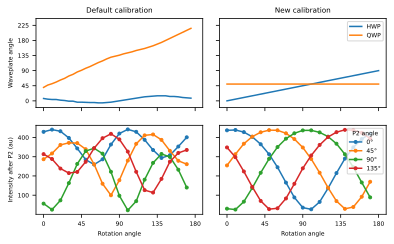
\includegraphics{detection_waveplate_calibrations.pdf}
	\caption{\todo{text}}
	\label{fig:detection waveplate calibrations}
\end{figure}

\todo{Mention the pol cube results.}

\section{Data analysis of conventional polarisation images}

\section{Polarisation-resolved STED microscopy (pSTED)}

\section{Samples used in this thesis}

	% !TeX spellcheck = en_GB
\chapter{Results}

\section{Demonstration of conventional polarisation microscopy}
\label{sec:conventional pol}

\begin{figure}
	\centering
	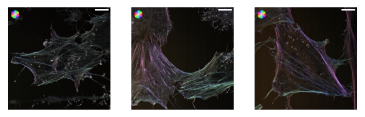
\includegraphics{conventional_pol.pdf}
	\caption{
		Polarisation microscopy images of three different cells. The colour wheel indicates the direction of polarised light corresponding to a certain colour. Scale bars \SI{10}{\mu m}. \todo{Get a camera view of with GFP and DAPI signals, see 21-02-05}
	}
	\label{fig:conventional pol}
\end{figure}

Even though we can't use polarisation on the detection side yet, we can already make polarisation images by varying the angle of excitation polarisation. As a proof of concept, I imaged the sample described in \autoref{sec:samples}, stepping the excitation light from \ang{0} to \ang{170} in steps of \ang{10}. Applying the algorithm detailed in \autoref{sec:pol analysis} to three different ROIs resulted in \autoref{fig:conventional pol}. As expected, vertically oriented fibres are excited by horizontal polarisation \cite{Spira2017}.

I also included power law scaling of the saturation (degree of polarisation) and value (total brightness) in the visualisation algorithm. These serve to adjust the brightness and contrast of the figure, as shown in \autoref{fig:power law exponents}.

\begin{figure}
	\centering
	\includegraphics{conventional_pol_exps.pdf}
	\caption{
		The effect of the exponents $ \alpha_s $ (tuning saturation) and $ \alpha_v $ (scaling brightness) on an image.
	}
	\label{fig:power law exponents}
\end{figure}

\todolist{
	\item I could plot some histograms and stuff, of the polarisation distribution, but I guess that only really makes sense if I can actually make a substantial comment about it.
	\item sSTED + polarisation
} 

\section{Polarisation-resolved STED microscopy}

In this section, I will detail how we implemented the pSTED scheme detailed in \autoref{sec:methods psted} and how we verified that it is working as predicted \todo{rephrase if conclusion is that it doesn't work ye}. The first step is to manipulate the polarisation of the depletion beam. Then I can do experiments on unpolarised and polarised controls (beads and Yersinia samples).

To get control of the light polarisation, the first step was to mount two new waveplates in the beam path. They were mounted after the SLM. A HWP was mounted inside a rotational stage and a QWP went in a cage system attached to the rotational stage, such that it is always aligned with the HWP, but that its rotational angle is fixed. The first step was to find the angle of the QWP that maximised the linearity of the light polarisation at the sample. This was simply done by placing a polariser and a power meter at the sample and rotating them to characterise the polarisation of the depletion beam. I did this a couple of times, from which we concluded that the optimal angle for the QWP was 15°. Next, I had to find the angle of the HWP at which the depletion beam is vertically polarised. In that position, the depletion beam has a polarisation parallel to the excitation lasers (at 0°). This turned out to be 38.4°. See \autoref{fig:psted hwp offset}. At a linearity of $ I_{max}/I_{min} = 5.47 $ (corresponding to an ellipticity $ \chi = \ang{10.3} $ )\todo{depends on definition of $ \chi $ again}, the polarisation of the linearised pSTED beam is comparable in quality to the 640 laser.

Now that we have control over the beam polarisation, we can check how the added waveplates influence the PSF. In \autoref{fig:psted psfs}, the PSF is shown for different polarisation directions. There are a number of conclusions we can draw from this data.  Firstly, the PSF is not radially symmetric any longer, even though the SLM was set to Gaussian mode. In particular, the ellipse orientation is parallel to the light polarisation, so we see the PSF rotating as we change the polarisation. This can be explained by the fact that a lens interacts differently with light polarised along different directions \cite{Egner2020}. This is the reason one should only use linearly polarised excitation light when performing polarisation microscopy.

Other effects of the polarisation include the following: the intensity of the depletion beam varies as a function of the polarisation angle. This is probably due to linear dichroism present in the optical elements between the waveplates and the sample. That is to be expected, but should be accounted during either image acquisition or analysis. Furthermore, the eccentricity of the ellipse has a slight dependency on the polarisation angle, and the maximum of the PSF moves a little: up to \todo{?} nm from its mean position. Fortunately this is a quite a bit below the diffraction limit for 775 nm light, i.e.~around 400 nm. \todo{Plot this data!}

\todo{NOTE THAT WE HAVE TO ROTATE THE HWP BACKWARDS!!!!!!!!}

Finally, we can perform pSTED on some control samples. I used two different ones: a sample of non-polarised beads and the cell sample shown earlier. Isotropic beads are useful, since we can determine the polarisation of emitted light by selectively activating fluorophores of a particular orientation with the polarisation of the excitation light. This process is called photoselection. When these beads are excited with circularly polarised light, fluorophores of all orientations should be activated equally, and the polarisation of the depletion beam should not matter. In the case of linearly polarised excitation light, on the other hand, depletion should be more efficient when its polarisation is aligned with the excitation beam. This can be verified by increasing the depletion power: when the beams are aligned, then the remaining fluorescence signal should drop faster than when they are not, as predicted by \autoref{eq:psted integral}. \autoref{fig:psted beads} shows that this is indeed the case. While there is some variation in the depletion rate under circular excitation, it can not be explained by the theory and seems random, unlike the case of linear excitation. There, depletion goes fastest when the beams are aligned, slower when there is a 45° angle between them, and slowest when they are orthogonal. If the depletion beam was more linearly polarised (i.e. had a lower $ \chi $), then this effect would be even more pronounced.

\begin{figure}
	\centering
	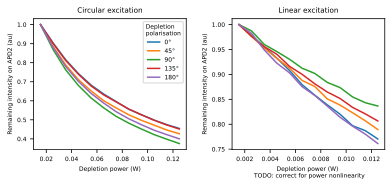
\includegraphics{psted_beads.pdf}
	\caption{
		Dependency of surviving fluorescence on intensity and polarisation of depletion beam. \textbf{Left:} circular excitation. \textbf{Right:} linear excitation at 0° (vertical). \todo{Planning to do a number of repeats to get rid of noise in this figure.}
	}
	\label{fig:psted beads}
\end{figure}

\todo{pSTED results in cells. Mention spacer channels. Mention that pSTED intensity shouldn't be too high, otherwise you'll never see anything.}





























	% !TeX spellcheck = en_GB

\chapter{Outlook}

\begin{itemize}
	\item Conventional polarisation microscopy
	\begin{itemize}
		\item Figure out detection waveplates, otherwise you can't use polarisation in the detection pathway
		
		\item I've made some measurements of polarisation sensitivities etc. We need to set up an analysis pipeline that makes use of them to correct systematic data errors before we can make quantitative statements about sample polarisation. Then we should really compare it to data from another lab and see if it matches.
		
		\item As part of that, tune the 640 and 775 waveplates to increase linearity to match the 561 laser.
		
		\item Improve the excitation waveplate calibration.		
	\end{itemize}

	\item Keep developing pSTED
	
	\item Other fancy polarisation stuff: FLIM + pol, FRET measurements, ...
	
	\item To do actual biological research, conventional pol microscopy is definitely the way to go. sSTED is easier than pSTED (for now).
\end{itemize}

\appendix

	\bibliographystyle{mystyle}
	\bibliography{other_sources,mendeley}
	
	% !TeX spellcheck = en_GB
\chapter{Acknowledgements}

Many thanks to Jason and Jonas for their great supervision. You have taught me so much, both academically and personally, and I feel extremely lucky that I got to do my thesis project with you guys. Thanks also to the others in the Tegenfeldt group: Elham, Esra, Oskar and Bao, for the good vibes and the occasional helping hand.

I am grateful to our collaborators in the Nordenfelt and Swaminathan groups, particularly to Valeriia, Swathi and Oscar who provided the samples I used throughout my project. To the polarisation community in Lund at large: thank you. I am grateful for the opportunity to organise our discussion sessions, which turned out the be instrumental to several parts of my thesis project.

A special mention goes out to Carl Troein. He has not been directly involved in this project, but as my programme coordinator, he has helped me navigate my new university and has helped me out a ton with getting a summer internship, which turned out to be a stepping stone to my next challenge.

I want to thank my friends and family for the continued support they gave me during this project, and simply for being part of my journey. Finally, I want to thank the Swedish public in general. I am extremely grateful for the opportunity to live in and discover your country for the past two years. It's been a blast!
%If there's anything I've learnt from my time here, it's this: \emph{det finns inget dåligt väder, bara dåliga kläder}.

\bigskip

\noindent Jonas, I promised you I'd share my star recipes, so check out the next page.
\newpage
\section*{Misir Wat}
\paragraph{Ingredients}
\begin{itemize}
	\item 4 tablespoons butter (or niter kibbeh, that's even better)
	\item 1 large yellow onion, very finely diced
	\item 3 cloves garlic, finely minced
	\item 1 tomato, very finely chopped
	\item 3 tablespoons tomato paste
	\item 2 tablespoons berbere, divided (you can get this at African Daily Market in Lund)
	\item 1 cup red lentils, rinsed
	\item 2.5 cups of vegetable stock
	\item 1 teaspoon salt
\end{itemize}

\paragraph{Preparation}
Melt 3 tablespoons of the butter in a medium stockpot.  Add the onions and cook over medium-high heat for 8-10 minutes until golden brown.  
Add the garlic, tomatoes, tomato paste and 1 tablespoon of the berbere and cook for 5-7 minutes. Reduce the heat if needed to prevent burning.
Add the broth and salt, bring it to a boil, reduce the heat to low and cover and simmer the lentils, stirring occasionally, for 40 minutes (adding more broth if needed) or until the lentils are soft.
Stir in the remaining tablespoon of butter and berbere. Simmer for a couple more minutes. Add salt to taste.
Serve with Ethiopian injeera, sourdough bread, or rice.

Source: \href{https://www.daringgourmet.com/misir-wat-ethiopian-spiced-red-lentils/}{\texttt{daringgourmet.com}}

\section*{Ginger Beer}

To start a ginger bug, combine 0.5 litres of water, 20 g of ginger (chopped or grated, but not peeled), and 28 g of sugar in a glass pot. Cover it with a clean towel and keep it at room temperature. Until it becomes fizzy, add 20 g of ginger and 30 g of sugar every day.

Then, combine 2 L of water, 200 g of sugar, and 75 g of ginger in a pot. Bring it to a boil, then reduce the heat and simmer for 5 to 8 minutes. Take it off the heat and let it cool down to room temperature. Add 100 g of strained ginger bug, and optionally some spices and the juice of three lemons. Divide over some airtight bottles and keep those at room temperature. Burp them daily by opening the cap to release built-up gas for about a week until the flavour is right and they are very carbonated. Then store them in the fridge for at least a couple of hours and enjoy!

Source: \href{https://www.joshuaweissman.com/post/fermented-ginger-beer}{\texttt{joshuaweissman.com}}

	\chapter{Code and data availability}

I've spent quite a bit of effort making this entire thesis easily reproducible from the raw data. To that end, the source code and data are published on GitHub, at \url{https://github.com/wduverger/msc-thesis}. If you want to generate all figures, you'll need to install a number of Python libraries in your environment (\ttfamily python-bioformats\rmfamily\ and \ttfamily python-opencv\rmfamily, among others). These packages have quite a lot of dependencies and can be tricky to install. If that is the case, or you just want to try to run the code without messing with your system too much, you can install Docker and build a container, a custom Linux virtual machine, with the Dockerfile in the GitHub repository.. 

If you experience any trouble setting this up, have any questions regarding this thesis or just want to chat about polarisation microscopy in general, do not be afraid to reach out! I am happy to help.
	\chapter{Characterisation and operation of the microscope}
\label{chap:characterisation}

This appendix gives more details on the optics of the microscope, with a focus on the polarisation state of light at different points in the beam paths. These are important for operating the setup, but less so for understanding the project as a whole.

\section{The laser modules}

The fast-switching 561~nm laser emits horizontally polarised light, but the polarisation can be tuned by three waveplates in its path. The last one, a quarter-wave plate, is fixed in its rotation angle. In the standard mode of operation, excitation laser light should be circularly polarised to minimise resolution reduction due to lens distortion etc.~\cite{Harke2008}. In that mode, the (fast or slow) axis of the first quarter-wave plate is aligned with the laser, such that it does not affect polarisation and the half-wave plate is set such that it rotates the (linearly polarised) light to \ang{45} with respect to the second quarter-wave plate. See \autoref{tab:laser polarisation} for the polarisation characteristics in the calibration provided by Abberior. The 561~nm laser is quite well-calibrated. In circular polarisation, it reaches a $ \chi$ very close to perfectly circular (\ang{45}).

The 640 nm laser does not have fast-switching built in, so instead, the light is fed into the microscope through a polarisation-preserving optical fibre by an acousto-optical modulator (AOM). The AOM is a crystal in the beam path, in which sound waves can be generated by a piezo element. The standing sound wave creates a diffraction grating with a variable pitch. That pitch is determined by the sound frequency, which can be modulated such that the first-order diffracted beam is either sent into the fibre aperture or not. The rest of the beam path is very similar to the 561 module, but the calibration of the waveplates in this pathway is not as accurate. Refer to \autoref{tab:laser polarisation}. 

The depletion laser travels through an entirely different set of optics than the excitation lasers to generate a donut beam. First, it travels through a half-wave plate that aligns the polarisation to the SLM (spatial light modulator). This HWP is necessary because an SLM adds an arbitrary spatially patterned phase delay to incident light, but only to the component polarised along its active axis. It will not alter the phase of the orthogonally polarised component. Using the proper phase delay patterns, one can create any (diffraction-limited) image in the sample plane. In this case, that would be a donut shape. Then -- ignoring the pSTED module for now, since that was not included in the original setup -- the beam travels through a half-wave plate to ensure circular polarisation in the sample plane (after going through a quarter-wave plate at \ang{45} to the QWP axes), just like the excitation lasers. This is done to ensure that the depletion efficiency does not depend on sample orientation and to avoid polarisation-dependent PSF distortion by lenses and other optics. The quality of the STED polarisation is similar to that of the 640 nm laser. Note that this is actually a significant result, since it means that the donut beam is not isotropically polarised. It will be far more effective at quenching fluorophores oriented along \ang{40} than those at \ang{130}.

\begin{table}
	\centering
	\begin{tabular}{lSSSS}
		\toprule
		Laser source     & {$ I_\mathit{max} / I_\mathit{min} $} & {$ \chi_I$ (deg)} & {$ \chi_E $ (deg)} & {$ \psi$ (deg)} \\ \midrule
		561 nm, linear (\ang{0})  & 23.6                              & 2.42                               & 11.6                               & 0                                \\
		561 nm, circular & 1.14                              & 41.2                               & 43.1                               & 20                               \\
		640 nm, linear (\ang{0})  & 6.13                              & 9.25                               & 22.0                               & 0                                \\
		640 nm, circular & 1.59                              & 32.2                               & 38.5                               & 120                              \\
		775 nm, circular & 1.61                              & 31.8                               & 39.2                               & 40                               \\ 
		775 nm, linear & 5.47 & 10.6 & 23.1 & 0 \\ \bottomrule
	\end{tabular}
	\caption{
		Polarisation characteristics of the lasers. Shown are linearity $ I_\mathit{max} / I_\mathit{min} $, ellipticity $ \chi_E $ ($ \chi_I$) of the electric field (intensity), and ellipse orientation $ \psi$ (anti-clockwise angle between ellipse orientation and vertical axis in sample plane). This data is based on \autoref{fig:laser polarisation}, except the linear setting of the 775 nm laser. This required fitting new waveplates, as explained later (\autoref{sec:psted implementation}).
	}
	\label{tab:laser polarisation}
\end{table}

\begin{figure}
	\centering
	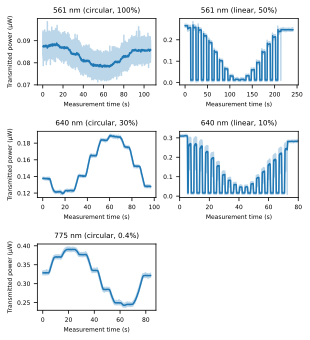
\includegraphics{laser_polarisation}
	\caption{
		Polarisation characterisation of the different lasers. To characterise circular polarisation, a polariser was placed in the sample and scanned from \ang{0} to \ang{180} in steps of \ang{20} (note that a sample is lacking at \ang{260} in the 775 nm data). Linear polarisation was characterised by fixing the polariser in place at \ang{0} and scanning the laser itself from \ang{0} to \ang{180} in steps of \ang{10}. Dark blue: average over 200 samples, light blue: raw data.
	}
	\label{fig:laser polarisation}
\end{figure}

One more thing we can derive from this data (see \autoref{fig:laser polarisation}), is that the 640 laser needs to ramp up every time it is powered on, due to the lack of fast switching.
This can be somewhat remedied in software by turning the laser ``on'', but at 0\% power. The effect of this is that the laser is on but the AOM directs laser light away from the fiber aperture, thereby shortening the time to ramp up the laser power. Furthermore, at low powers, the laser intensity may not be proportional to the power setting in software. Their actual relationship is shown in \autoref{fig:laser power}. If experiments need to be done at low power, a neutral density filter is required. This is luckily not the case for biological specimens with a low density of fluorophores.

\begin{figure}[ht]
	\centering
	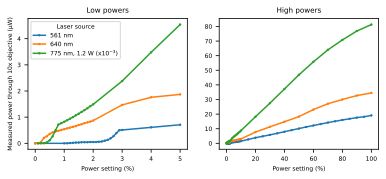
\includegraphics{laser_power}
	\caption{
		The power of each of the three lasers as measured through a 10x objective. Notice the non-linearity at low power settings. The 775 nm data was scaled down by three orders of magnitude.
	}
	\label{fig:laser power}
\end{figure}

Looking at the calibrations of the waveplates in the excitation modules (\autoref{fig:excitation waveplate calibration}), one can see that they move quite erratically, but they do work, as shown in \autoref{fig:laser polarisation}. This could be an effect of the automated calibration performed by Abberior. In the 561 nm calibration, for example, one can see that the QWP constantly flips between about \ang{30} and \ang{120}, which are \ang{90} apart. The calibration works, but the eccentricity of the polarisation ellipse depends on the orientation. In other words, for a more rigorous characterisation of the microscope, \autoref{tab:laser polarisation} should have an entry for every possible calibration setting.

\begin{figure}
	\centering
	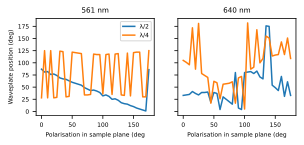
\includegraphics{excitation_waveplate_calibrations.pdf}
	\caption{
		Calibrations of the excitation waveplates, as supplied by the microscope manufacturer.
	}
	\label{fig:excitation waveplate calibration}
\end{figure}

One can measure the PSFs of the lasers by scanning over a reflective gold bead and acquiring an image on the photomultiplier tube (PMT). These are shown in \autoref{fig:normal psfs}.

\begin{figure}
	\centering
	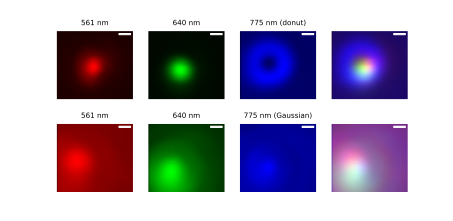
\includegraphics{laser_psfs.pdf}
	\caption{
		Point spread functions of the different lasers (in donut and Gaussian modes) at different SLM configurations, by measuring the reflection from 100 nm wide gold beads.
	}
	\label{fig:normal psfs}
\end{figure}

\section{The detection module}

The main detectors of the microscope are a set of avalanche photodiodes (APDs), but there is also a highly sensitive PMT right after the QWP on the microscope end. The PMT is usually used to measure the point spread functions of the lasers and to align them with each other. In normal operation, the light travels on to the detection waveplates, then through a pinhole wheel, passes filters and dichroic mirrors in the filter cube housings, and is finally reflected onto the APDs. The wheel contains pinholes of different sizes, which allows for choosing the trade-off between light collection and $ z $ resolution, depending on the quality of the sample. Different filter cubes are available with various bandpass filters, dichroic mirrors, and/or a polarising beam splitter (PBS).

The APDs show a slight polarisation sensitivity of about 10\% (see \autoref{fig:apd pol sensitivity}). I measured this by exciting Tetraspec beads with the 561 laser set to circular excitation, such that the emission light is non-polarised. Then I placed a linear polariser behind the detection waveplates and measured their signal as a function of the polariser angle. It seemed like the beam moved depending on the incident polarisation, as aligning the APDs when the signal was minimal did help a little, but the imperfect circularity of the 561 laser may also play a role, as it is on the same order of magnitude. 

\begin{figure}
	\centering
	\includegraphics{apd_pol_sensitivity.pdf}
	\caption{Dependence of the signal from APD1 on the angle of polarisation of incoming light.}
	\label{fig:apd pol sensitivity}
\end{figure}

\subsection{Calibrating the detection waveplates}

We did have some problems with the waveplates in the detection module. They can be controlled through Abberior's software suite (Imspector), but it is not clear if they are set up correctly. The calibration is based on a control angle that I will denote $ \theta $. It would theoretically be possible for this setup to rotate polarised light of any orientation, since
\begin{equation}
	S_\hwp(\theta/2) S_\qwp(0) S_\qwp(0) = \mqty(\cos\theta & -\sin\theta \\ \sin\theta & \cos\theta ),
	\label{eq:detection waveplates}
\end{equation}
which is simply the rotation matrix $ R(\theta) $. The exact position of the quarter-wave plates does not matter, as long as they are aligned with each other. If the waveplates are at an angle $ \phi$ instead of 0, then this set of waveplates rotates the polarisation by an angle $ (\theta-2\phi) $ instead. 

It is unclear what goal the original calibration (see \autoref{fig:detection waveplate calibrations}) should serve. If we approximate the default calibration with a QWP at $ \theta $ and a HWP at 0, then the action of these waveplates would be
\begin{equation}
	S_\hwp(0)\cdot S_\qwp(\theta)\cdot S_\qwp(0) = 
		\mqty( \cos^2\theta + i\sin^2\theta & (1+i)\cos\theta\sin\theta \\
			   (-1+i)\cos\theta\sin\theta   & \cos^2\theta - i\sin^2\theta 
	    ).
\end{equation}

Therefore, I developed a new calibration. To do so, I first needed to establish at what angle the second quarter-wave plate would be aligned to the first one. I did this by placing a polariser in the sample holder (P1) and illuminating it with the top lamp, such that the light incident on the first quarter-wave plate was linearly polarised. Then I placed another polariser (P2) after that waveplate (i.e.~before the last two waveplates) that I rotated to assess the linearity of the polarisation there. I found the angle of P1 at which light was most circular after the first QWP and subsequently placed P2 after all waveplates to find the angle of the second QWP that would make the polarisation linear again. At this point, the QWPs should be aligned. They could also be at \ang{90} to one another. To distinguish between these setups, compare a measurement such as \autoref{fig:p1 effects} with simulations in \autoref{fig:detection waveplate simulations}.

\begin{figure}
	\centering
	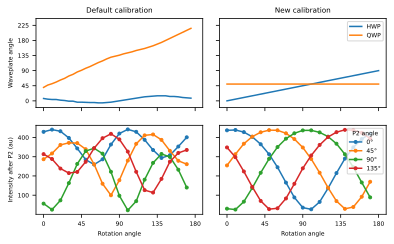
\includegraphics{detection_waveplate_calibrations.pdf}
	\caption{
		A comparison of the default detection waveplate calibration and the new one. The new calibration seems to actually rotate incident polarisation by an arbitrary angle.
	}
	\label{fig:detection waveplate calibrations}
\end{figure}


\begin{figure}
	\centering
	\includegraphics[scale=.95]{p1_effects_qwp_aligned.pdf}
	\includegraphics[scale=.95]{p1_effects_qwp_30.pdf}
	\includegraphics[scale=.95]{p1_effects_qwp_90.pdf}
	\caption{
		Simulation of the effect of QWP alignment on the action of the detection pathway. Shown are three simulations in which the first QWP is rotated by 0, 30, and 90 degrees, respectively. The second QWP is always rotated by 0, and the HWP is rotated to half the rotation angle (x-axis). When the QWPs have an offset of 90 degrees (bottom), the upper and lower panels (with either P1 or P2 constant) are identical, but when they are aligned (top), there is a phase difference. When they are not aligned at all (middle), intensity variations are prominent. This simulation is based on \autoref{eq:detection waveplates}.
	}
	\label{fig:detection waveplate simulations}
\end{figure}


Second, I assessed both calibrations. As presented in \autoref{fig:detection waveplate calibrations}, the new calibration works rather well, unlike the original one. However, its performance seems to depend on the precise angle of P1, see \autoref{fig:p1 effects}.
This needs to be fixed before we can confidently use polarisation-affecting elements in the detection path. Luckily, simulations show that this effect can be explained by misalignment between the QWPs. Therefore, a more accurate calibration should fix this problem.

\begin{figure}[h]
	\centering
	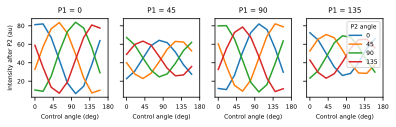
\includegraphics{p1_effects.pdf}
	\caption{
		The effect of rotating the incoming polarisation (P1). The detection waveplates seem to rotate the polarisation for P1 at \ang{45} or \ang{135}, but seem to circularise incoming light at \ang{0} and \ang{90} somewhat. (Note that the angle of P1 does not have a proper reference since I forgot to home the rotator.)
	}
	\label{fig:p1 effects}
\end{figure}


Finally, I checked the POL cube, which contains a polarising beam splitter (PBS) and some wavelength filters. It seems to work as expected (see \autoref{fig:pol cube}). The transmitted ray has an extinction ratio of about 0.2, meaning that 20\% of the power of rays that are orthogonally polarised to the transmission axis (and hence should be reflected by the PBS) is actually transmitted. On the other hand, it has an extinction ratio of .01 for the reflected wave.

\begin{figure}
	\centering
	\includegraphics{pol_cube.pdf}
	\caption{Performance of the polarising beam splitter.}
	\label{fig:pol cube}
\end{figure}

\section{Protocol for polarisation microscopy}
\label{sec:polarisation microsocpy protocol}

After acquisition, a stack of images $ I_{nxy} $ (with excitation light polarised along $ \theta_n $) must go through a number of steps to be converted into a false-colour polarisation image. Those steps are detailed in this section.

\subsection{Stack alignment.} Images in a stack are aligned using an ECC (enhanced correlation coefficient) optimisation algorithm implemented in OpenCV, an open source computer vision library, which optimises an adjusted version of the correlation between two images, subject to certain constraints, e.g.~translation, without shearing or rotation \cite{Evangelidis2008}. When the correlation between two images is maximised, they are aligned. The innovation of the ECC algorithm lies in the definition of an enhanced correlation coefficient which requires less computational power and is more robust than other algorithms \cite{Evangelidis2008}. 

If the goal is to generate a new image stack $ I'_{nxy} $, corrected for sample or beam drift, we can take the first frame as reference, setting 
\begin{equation}
	I'_{0xy} = I_{0xy}.
\end{equation}
For every other frame $ I_{nxy} $, we can calculate a warp matrix using OpenCV with the \texttt{findTransformECC()} method, which maximises the correlation between $ I_{nxy} $ and $ I'_{(n-1)xy} $. Since we only observe drift in the images, we only allow translation (no shearing or rotation). Finally, we transform the original image using that warp matrix and \texttt{warpAffine()} and save the result as $ I'_{nxy} $.

\noindent In other words:
\begin{equation}
	I'_{nxy} = \texttt{warpAffine}\left(
		I_{nxy},\,
		\texttt{findTransformECC}\left(I'_{(n-1)xy}, I_{nxy}\right)
	\right),
\end{equation}
for all $ n>0 $.

\subsection{Bleaching compensation.} Since photobleaching will influence the calculation of the Fourier coefficients, it needs to be separated from the polarisation response. We can estimate the bleaching rate from the ratio between two frames at identical polarisations. Unfortunately, the Imspector software suite does not allow for rotating the excitation polarisation by more than \ang{175}, so we cannot do this exactly. It would be possible if we were able to use the POL cube, but that is not an option, as explained before. Let $ \bar{I}_0 $ be the mean intensity of the first image, and $ \bar{I}_N $ the mean intensity of the last one. For now, we simply estimate the bleaching per frame as
\begin{equation}
	r = \left( \frac{\bar{I}_N}{\bar{I}_0} \right) ^{1/N},
\end{equation}
given $ N+1 $ number of frames were acquired. Then we can compensate for photobleaching by multiplying every frame with a correction factor as
\begin{equation}
	I''_{nxy} = r^{-n} I'_{nxy}.
\end{equation}

\subsection{Colouring the image.} For every pixel, calculate a complex-valued Fourier coefficient corresponding to a period of \ang{180} (at which we should see polarisation dependence) using
\begin{align}
	F_{xy} &= \sum_n I''_{nxy} e^{i2\theta_n}.
\end{align}
Then construct an image in HSV colour space where 
\begin{align}
	h_{xy} &= \arg (F_{xy}),\\
	s_{xy} &= \abs{F_{xy}}/v_{xy},\\
	v_{xy} &= \sum_n I_{nxy}.
\end{align}
Finally, normalise every channel $ c $ to be in the range $ (0,1) $ and optionally apply a power law with a manually chosen coefficient $ \alpha_c $ for optimal visualisation,
\begin{equation}
	c'_{xy} = \left( \frac{c_{xy}}{\max c_{xy}} \right)^{\alpha_c}.
\end{equation}
The effect of $ \alpha_c $ is presented in \autoref{sec:conventional pol}. If necessary, the Fourier image $ F_{xy} $ can be blurred before constructing a false colour image. This can be useful when the image is too noisy for a decent Fourier calculation.

\section{pSTED optics}

\label{sec:psted implementation}

The system was not set up to offer control over the depletion polarisation. Instead, the STED polarisation is always circular, and this is ensured by a set of two fixed waveplates: a QWP and a HWP (refer to \autoref{fig:layout} and the description of the STED module in that section). 

To control the polarisation of the depletion beam for pSTED, I first had to linearise the polarisation by compensating for the QWP in the beam path. That can be done by placing a QWP in the pSTED module in \autoref{fig:layout}, since
\begin{equation}
	S_\qwp(\phi)S_\hwp(0)S_\qwp(-\phi) = R(2\phi).
\end{equation}
When the quarter-wave plates are aligned like that (when they are each others mirror image with respect to the HWP fast axis), this system simply rotates the polarisation by a fixed angle. This means that adding a HWP before this setup suffices to get full control over the polarisation angle of the depletion beam.

\begin{figure}
	\centering
	\includegraphics[height=.35\linewidth]{psted optics 1.jpg}%
	\hfill%
	\includegraphics[height=.35\linewidth]{psted optics top.jpg}
	\caption{
		The new pSTED optics. The rotational stage holds a HWP and a stationary QWP is mounted on a cage system. To take these optics out of the microscope, only the screw that holds the foot needs to be removed.
	}
	\label{fig:psted optics photo}
\end{figure}

In practice, the first step was to mount these two new waveplates in the beam path. They were mounted right after the SLM on an easily removable foot, see \autoref{fig:psted optics photo}. This way, conventional STED and polarisation-dependent STED are both easily performed. The HWP was mounted inside a rotational stage and the QWP in a cage system attached to the rotational stage, such that it is always aligned with the laser beam, but that its rotational angle is fixed. The first step was to find the angle of the QWP that maximised the linearity of the light polarisation at the sample. This was done by placing a polariser and a power meter at the sample and rotating them to characterise the polarisation of the depletion beam. I did this a couple of times, from which we concluded that the optimal angle for the QWP was \ang{15}. Next, I had to find the angle of the HWP at which the depletion beam is vertically polarised. In that position, the depletion beam has a polarisation parallel to the excitation lasers (at \ang{0}). This turned out to be \ang{38.5} (or equivalently $\ang{38.5}+\ang{180}=\ang{218.5}$). See \autoref{fig:psted hwp offset}. At a linearity of $ I_{max}/I_{min} = 5.47 $, the polarisation of the linearised pSTED beam is comparable in quality to the 640 laser (see \autoref{tab:laser polarisation}). Note that the HWP angle $ \theta_\hwp $ must satisfy
\begin{equation}
	\theta_\hwp = \ang{218.5} - \theta/2
\end{equation} 
to achieve a linear polarisation along $ \theta $ in the sample plane.

\begin{figure}
	\centering
	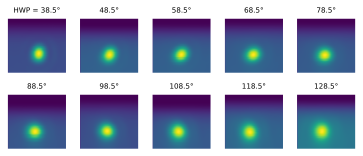
\includegraphics{psted_psfs.pdf}
	\caption{
		Depletion PSF as a function of beam polarisation. The figure titles indicate the angle of the new HWP. The shown images are recentred on the pixel with the highest intensity to correct for displacement.
	}
	\label{fig:psted psfs}
\end{figure}

Now that we have control over the beam polarisation, we can check how the new waveplates influence the PSF. In \autoref{fig:psted psfs}, the PSF is shown for different polarisation directions. There are several conclusions we can draw from this data.  Firstly, the PSF is not radially symmetric any longer, even though the SLM was set to Gaussian mode. (This is easy to do. It only requires removing the donut-generating pattern on the SLM.) In particular, the ellipse orientation is parallel to the light polarisation, so we see the PSF rotating as we change the polarisation (see also \autoref{fig:psted psf orientation and power}). This can be explained by the fact that lenses interacts differently with light polarised along different directions \cite{Egner2020}. This is the reason one should only use linearly polarised excitation light when performing polarisation microscopy.

Other effects of the polarisation include the following: the intensity of the depletion beam varies as a function of the polarisation angle (see \autoref{fig:psted psf orientation and power}). This is probably due to linear dichroism present in the optical elements between the waveplates and the sample. This is not a surprising result, but should be accounted for during either image acquisition or analysis. Furthermore, the maximum of the PSF moves a little: up to roughly 100~nm from its mean position (\autoref{fig:psted displacement}). Fortunately, this is quite a bit below the diffraction limit for 775 nm light, i.e.~around 400 nm, so the effect will be rather small.

\begin{figure}
	\centering
	\includegraphics{psted_hwp_offset.pdf}
	\caption{
		The new rotating HWP in the pSTED module controls the depletion beam polarisation. With an offset of 38.5°, the depletion beam is parallel to the 640 laser (set to vertical linear polarisation).
	}
	\label{fig:psted hwp offset}
\end{figure}

\begin{figure}
	\centering
	\includegraphics{psted_psfs_orientation_and_power.pdf}
	\caption{
		\textbf{Left:} The pSTED PSF is elliptical, and its orientation matches the light polarisation. \textbf{Right:} pSTED intensity depends on polarisation. Error bars show standard deviation, n=10.
	}
	\label{fig:psted psf orientation and power}
\end{figure}

\begin{figure}
	\centering
	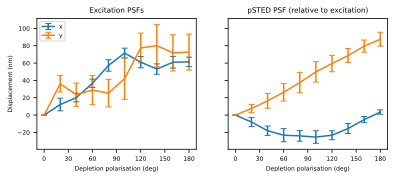
\includegraphics{psted_psfs_displacement.pdf}
	\caption{
		The displacement of the laser PSFs as a function of depletion polarisation. \textbf{Left:} The displacement of the 561~nm and 640~nm PSFs (representing drift in the image). \textbf{Right:} Displacement of the pSTED PSF relative to the excitation PSFs.
	}
	\label{fig:psted displacement}
\end{figure}
	% !TeX spellcheck = en_GB

\chapter{A note on laser safety}

The \SI{775}{nm} line is a class 4 laser source. Under normal operation, the user is protected from it. However, when calibrating the STED beam or placing new components in the beam path, it is theoretically possible for the collimated laser beam to be reflected into the user's eyes. A high-powered laser beam can do permanent damage to the skin and retina, so we have to make sure we stay below the limits imposed by the Work Environment Agency's (Arbetsmiljöverkets) limits \cite{AFS2009:7}. These regulations set forth three main conditions to calculate the Maximum Permissible Exposure (MPE) of a pulsed laser, see table 2.6 of the regulations. Important values and formulas about our setup, as well as the limits provided by the Work Environment Agency are provided in \autoref{tab:laser-safety} and in the text below.

\begin{table}[h]
	\centering
	\caption{Operating characteristics of the 775 laser line and relevant safety parameters. }
	\begin{tabular}{lll}
		\toprule
		Quantity                   & Symbol               & Value                 \\ \midrule
		Beam radius                & $ r $                & 0.5 mm                \\
		Pulse width (FWHM)         & $ \tau $             & 1.3 ns                \\
		Pulse repetition frequency & $ f $                & 40 MHz                \\
		Pulse energy               & $ E_\mathit{pulse} $ & 31 nJ                 \\
		Average power              & $P_\mathit{avg} $    & 1.25 W                \\ \\
		Thermal correction time    & $ T_\mathit{min} $   & 18 \si{\micro\second} \\
		Ca                         & $ C_a $              & 1.41                  \\
		Cc                         & $ C_c $              & 1                     \\
		Ce                         & $ C_e $              & 1                     \\ \bottomrule
	\end{tabular}
	\label{tab:laser-safety}
\end{table}

\paragraph{Rule 1: The dose of a single pulse must not exceed the single-pulse MPE.} The pulse dose $ H_\mathit{pulse} $ of the 775~nm laser at full power is
\begin{equation}
	H_\mathit{pulse} = \frac{E_\mathit{pulse}}{2\pi r^2} \approx \SI{39}{mJ/m^2},
\end{equation}
whereas the MPE equals
\begin{equation}
	H_\mathit{pulse}^\mathit{MPE} = \num{5e-3} C_a C_e = \SI{7.1}{mJ/m^2}.
\end{equation}
This formula is found in table 2.2 of the regulations.

\paragraph{Rule 2: The dose of a single pulse may not exceed the thermally-corrected MPE.} This weighs the pulse MPE with the amount of pulses in an interval $ T_\mathit{min} $. The number of pulses in such an interval is $ n = f\cdot T_\mathit{min} $, so
\begin{equation}
	H_\mathit{thermal}^\mathit{MPE} =  n^{-1/4} H_\mathit{pulse}^\mathit{MPE} = \SI{1.3}{mJ/m^2}.
\end{equation}
Rule 2 is therefore more strict than the rule 1. For safe operation, the laser must be ran at a power below 3.3\% $ (=H^\mathit{MPE}_\mathit{thermal} / H_\mathit{pulse}) $.

\paragraph{Rule 3: The cumulative dose for a group of pulses in an interval of time t must not exceed the MPE for a single pulse of that time.} Taking the necessary values from tables 2.2 and 2.3, the cumulative MPE is defined as
\begin{equation}
	H_\mathit{tot}^\mathit{MPE}(t) = \left\{\begin{array}{rl}
		\num{5e-3} \:C_a C_e &  t<\SI{18}{\mu s,} \\
		18 t^{0.75} \:C_a C_e &  \SI{18}{\mu s} < t < \SI{10}{s}, \\
		10 t\:C_a C_c  &t> \SI{10}{s}.
	\end{array}\right.
\end{equation}
The actual dose, on the other hand, is
\begin{equation}
	H_\mathit{tot}(t) = \lfloor ft \rfloor H_\mathit{pulse},
\end{equation}
where $ \lfloor \cdot \rfloor$ is the flooring function. This function is plotted in \autoref{fig:laser-safety-mpe}, from which it can be seen that the laser is only safe to use at 0.0005\% capacity. Since the minimum laser power offered by the software is .05\%, OD2 goggles should be worn to guarantee safe operation of the 775~nm laser.

\begin{figure}
	\centering
	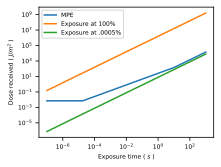
\includegraphics{laser_safety.pdf}
	\caption{Maximum permissible  and actual exposure to the collimated STED beam as a function of exposure time.}
	\label{fig:laser-safety-mpe}
\end{figure}

\end{document}
